\section{3D mesh fitting}

\subsection{Designing a better filter}

The previous approach for cross-correlation described in Section \ref{sec:CC} relies purely on matching filled voxels.
It suffers from the problem that the filter tends to fit better when aligned diagonally across both legs - in the position where it can match the greatest number of voxels.
To correct this problem we can create a new filter that is more intelligent about the type of voxels it matches.

\begin{figure}[b]
	\centering
	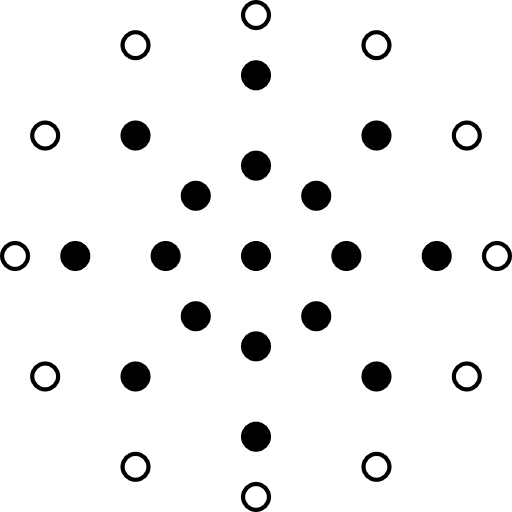
\includegraphics[width=4cm]{../interim/improvedfilter.png}
	\caption{A cross section through the improved cross-correlation filter.
		Black circles represent filled voxels, and white circles represent edge voxels.}
	\label{ImprovedFilterCross}
\end{figure}

Instead of points in the filter having an intensity value $i \in \{0 \cdots 1\}$, our points could take one of two possible states: they could match either an edge voxel or a filled voxel.
This would hopefully overcome the problem of a filter spanning the two legs, as the area between the legs would contain edge voxels.
These edge voxels wouldn't match up with the edge-seeking points in the new filter, and so would be a lower match than if the filter was placed the proper position on the thigh.

\begin{figure}[tb]
	\centering
	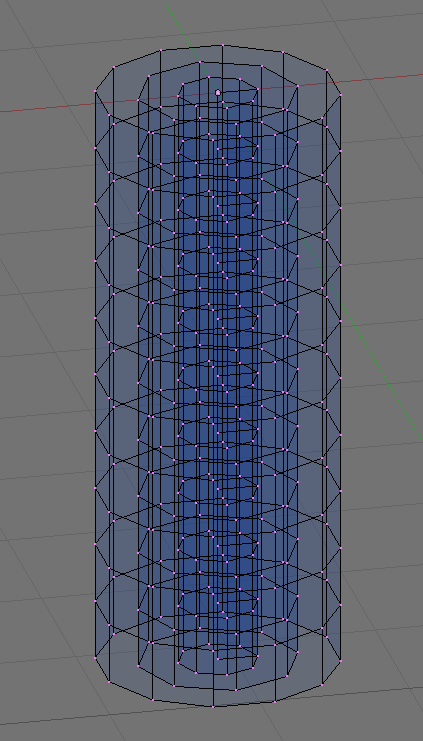
\includegraphics[width=5cm]{thighmodel.png}
	\caption{The cross-correlation filter rendered in the Blender application.
		Although not shown in this image, the outer points in the mesh are coloured white to indicate that they should
		match only edge voxels.}
	\label{ImprovedFilter}
\end{figure}

Figure \ref{ImprovedFilterCross} shows a cross section of such a filter.
It can be seen that the filter contains two types of points - those around the outside that should match edge voxels,
and those in the middle that should match filled voxels through the centre of the thigh.

One important thing to consider about this idea is whether the points in the filter should be spaced in a regular grid.
In the form shown in Figure \ref{ImprovedFilterCross} the points have an arbitrary spacing and are very different from the original filter shown in Figure \ref{ThighFilterCrossSections}.
A filter with points arranged in a regular grid is not necessarily advantageous when matching against discrete voxel data due to the rotations and transformations that the filter will undergo.
In the process of finding the best fitting with the data the filter will be scaled to fit the proportions of the subject, and rotated to match the angle of the leg.
By doing this any one-to-one relationship between pixels in the filter and voxels in the sample data will be lost.

Since there is no advantage to be gained from using a regularly spaced filter, it was decided that a better form for the filter would be that of a mesh.
The final mesh was designed using Blender \cite{Blender} and can be seen in Figure \ref{ImprovedFilter}.



\subsection{Matrix transformations}

In order to match the filter mesh to the voxel data, a matrix would need to be defined that transforms the points from their positions
in mesh-space to their new positions in the voxel-space.
The standard matrix transformations listed in Appendix G of the OpenGL Red Book \cite{RedBook} were used:

\begin{equation}
	\mathbf{M}_{trans}(v) =
	\left(\begin{array}{cccc}
		1 & 0 & 0 & v_{x} \\
		0 & 1 & 0 & v_{y} \\
		0 & 0 & 1 & v_{z} \\
		0 & 0 & 0 & 1
	\end{array} \right)
\end{equation}

\begin{equation}
	\mathbf{M}_{scale}(v) =
	\left(\begin{array}{cccc}
		v_{x} & 0 & 0 & 1 \\
		0 & v_{y} & 0 & 1 \\
		0 & 0 & v_{z} & 1 \\
		0 & 0 & 0 & 1
	\end{array} \right)
\end{equation}

\begin{equation}
	\mathbf{M}_{rotx}(\phi) =
	\left(\begin{array}{cccc}
		1 & 0 & 0 & 0 \\
		0 & cos(\phi) & -sin(\phi) & 0 \\
		0 & sin(\phi) & cos(\phi) & 0 \\
		0 & 0 & 0 & 1
	\end{array} \right)
\end{equation}

\begin{equation}
	\mathbf{M}_{roty}(\phi) =
	\left(\begin{array}{cccc}
		cos(\phi) & 0 & sin(\phi) & 0 \\
		0 & 1 & 0 & 0 \\
		-sin(\phi) & 0 & cos(\phi) & 0 \\
		0 & 0 & 0 & 1
	\end{array} \right)
\end{equation}

\bigskip
First the size of the filter is normalised - scaling all the vertices so they lie in the range ${0 \cdots 1}$.
It is assumed that the origin of the model's coordinate system is already in the centre of its top face.

\begin{equation}
	\mathbf{M}_{1} = \mathbf{M}_{scale}(\frac{1}{\max \{\text{modelSize}_{x}, \text{modelSize}_{y}, \text{modelSize}_{z} \}})
\end{equation}

Then the filter is scaled up to voxel-space.
$h$ is the height of the subject as determined in Section \ref{LocatingCenter}.
We assume that the length of the thighs and lower legs are equal, and are a quarter of the subject's total height.

\begin{equation}
	\mathbf{M}_{2} = \mathbf{M}_{scale}(\frac{h}{4}, \frac{h}{4}, \frac{h}{4})
\end{equation}

Next we apply the relevant rotations to the limbs.
The angles $\theta$ and $\alpha$ used here are the same as in Section \ref{sec:CC} -
$\theta$ is the rotation of the leg along the direction of movement and $\alpha$ is the rotation perpendicular to the direction of movement.

\begin{equation}
	\mathbf{M}_{5} = \mathbf{M}_{rotx}(\theta_{1}) * \mathbf{M}_{roty}(\alpha_{1})
\end{equation}

We now move the mesh to the estimated position of the subject's leg.
Equation \ref{eqn:TransToHip} translates the mesh to the centre of the hip, and equations \ref{eqn:TransToRightLeg} and \ref{eqn:TransToLeftLeg} perform additional
translations to the right or left leg position respectively.
As determined in Section \ref{LocatingCenter} $w$ is the width, or extent along the x axis, of the subject,
and $\mathbf{V}_{mean}$ is the mean filled voxel position.

\begin{align}
	\label{eqn:TransToHip}      \mathbf{M}_{6}  &= \mathbf{M}_{trans}(\mathbf{V}_{mean_{x}}, \mathbf{V}_{mean_{y}}, \frac{h}{2}) \\
	\label{eqn:TransToRightLeg} \mathbf{M}_{7r} &= \mathbf{M}_{trans}(+\frac{w}{6}, 0, 0) \\
	\label{eqn:TransToLeftLeg}  \mathbf{M}_{7l} &= \mathbf{M}_{trans}(-\frac{w}{6}, 0, 0)
\end{align}

Now armed with the above set of transformations, we are able to move the points in our mesh into the correct location in the voxel-space:

\begin{equation}
	\label{eqn:Thigh} \mathbf{M}_{thigh} = \mathbf{M}_{7} * \mathbf{M}_{6} * \mathbf{M}_{5} * \mathbf{M}_{2} * \mathbf{M}_{1}
\end{equation}

You may notice that we have missed out $\mathbf{M}_{3}$ and $\mathbf{M}_{4}$.
Equation \ref{eqn:Thigh} describes the transformation for each of the thighs.
An additional two matrix transformations can be introduced to account for the lower legs:

\begin{align}
	\mathbf{M}_{3} &= \mathbf{M}_{rotx}(\theta_{2}) * \mathbf{M}_{roty}(\alpha_{2}) \\
	\mathbf{M}_{4} &= \mathbf{M}_{trans}(0, 0, -\frac{h}{4})
\end{align}

Again we are using $\alpha$ and $\theta$ to refer to the angles the lower legs make with the vertical.
These equations give us a composite transformation that describes the lower legs:

\begin{equation}
	\label{eqn:LowerLegs} \mathbf{M}_{lowerleg} = \mathbf{M}_{7} * \mathbf{M}_{6} * \mathbf{M}_{5} * \mathbf{M}_{4} * \mathbf{M}_{3} * \mathbf{M}_{2} * \mathbf{M}_{1}
\end{equation}



\subsection{Fitting to the data}

In our previous approach in section TODO, a program would iterate over all the pixels in the filter and sample the
voxel data in the corresponding location.
The value of the filter (a real number between 0 and 1) would be multiplied by the value of the voxel (integer 0 or 1 - representing empty or filled) to produce a ``score''.
The scores of all these samples would then be summed to produce the final fitting score for that orientation.

A better approach would be a more traditional linear regression method such as least squares, as used by Zhihui et al. \cite{LinearModelFitting}.
Figure \ref{FittingImages} shows a two-dimensional example to demonstrate this least squares fitting, however three dimensional fitting works in exactly the same way.
The goal is to fit a mesh (shown as black dashed lines) to voxel data in the shape of a leg (shown as a filled green rectangle).
The mesh contains a number of nodes which are shown in the diagrams as filled circles.
Yellow circles are trying to match edge voxels, and blue circles are trying to match filled non-edge voxels.

\begin{figure}[tb]
	\centering
	\subfloat[High energy fitting]{\label{FittingImageHigh}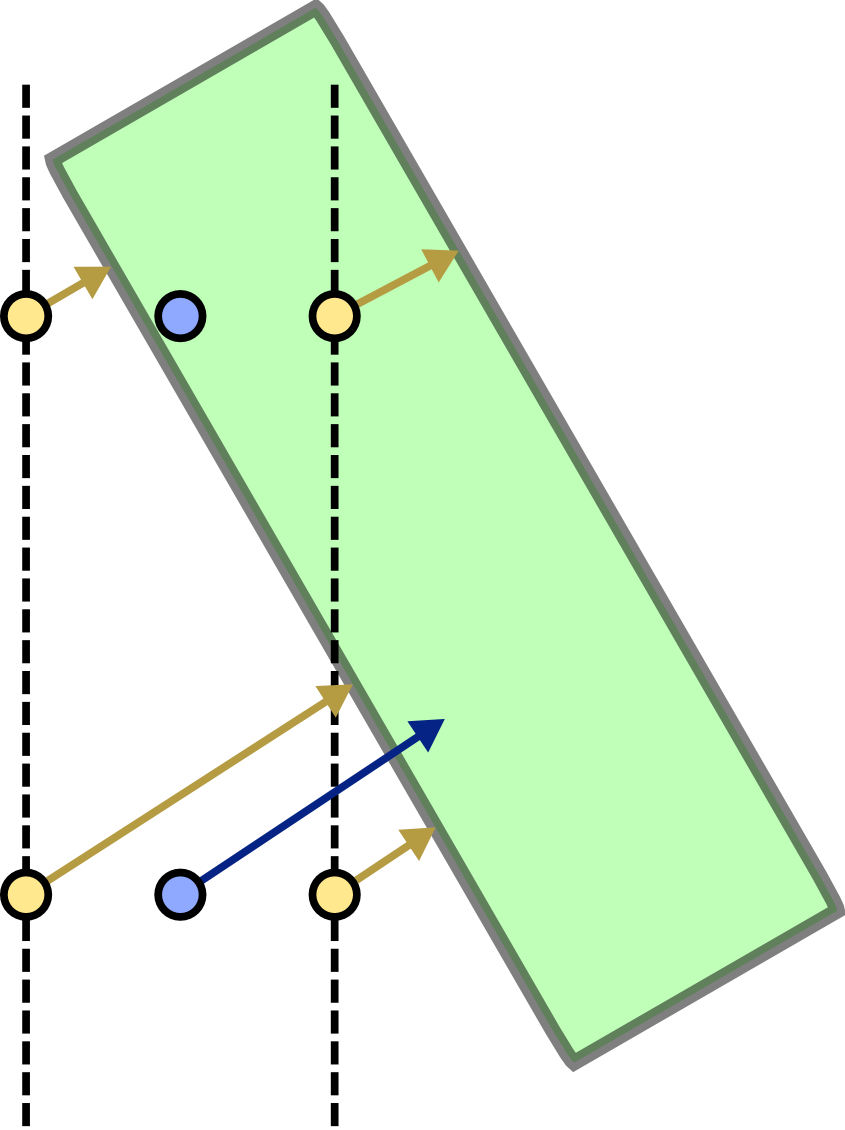
\includegraphics[height=6cm]{fitting1.png}}
	\qquad
	\subfloat[Low energy fitting]{\label{FittingImageLow}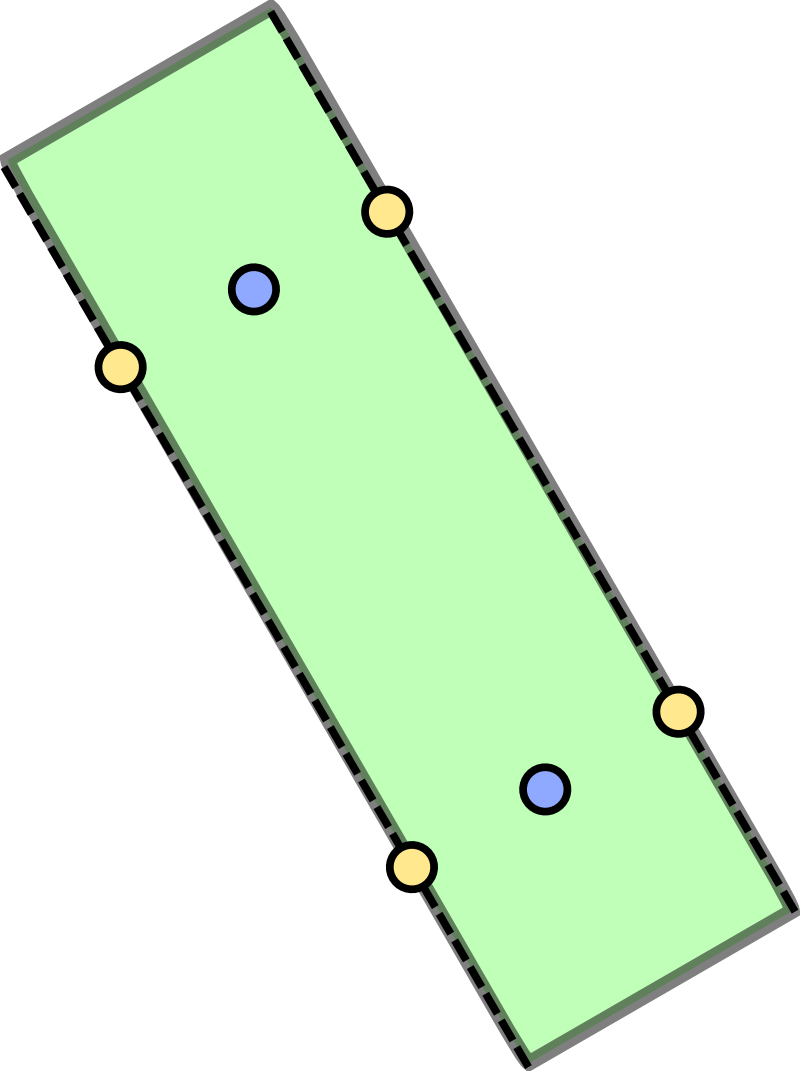
\includegraphics[height=6cm]{fitting2.png}}
	\caption{Potential fittings of our mesh filter.
		The filled green rectangle represents the voxels of a subject's thigh,
		and the coloured circles show a few of the nodes in the mesh.}
	\label{FittingImages}
\end{figure}

An algorithm iterates over the six nodes in the mesh, and for each one searches for the nearest suitable voxel (for the yellow nodes, only edge voxels are suitable).
The first potential fitting, Figure \ref{FittingImageHigh}, has the mesh orientated straight down ($\theta = 0$) and only one of the nodes - the blue one at the top - lies directly on top of a suitable voxel.
The sum of the squared distances between each of the nodes and its closest suitable voxel is taken, and this is used as the overall ``energy'' of that orientation.
Figure \ref{FittingImageHigh} has a high energy as the distances between the nodes and their voxels is very large.
Figure \ref{FittingImageLow} has an energy of $0$, as each node lies directly on top of a suitable voxel.

To find the parameters that give the best fit for an individual frame, one approach would be to iterate over all possible parameters and accept the one that has the least energy.
Such an implementation is shown in Listing \ref{leastsquarescode}.

\begin{lstlisting}[firstnumber=1,language=c,morekeywords={step,function,foreach,in},frame=single,mathescape=true,caption={Least squares fitting pseudo-code},label={leastsquarescode},float=[tb]]
function fit
	$range_\theta = \frac{\pi}{4}$
	$range_\alpha = \frac{\pi}{32}$
	$resolution_\theta = 41$
	$resolution_\alpha = 11$
	
	$bestEnergy$ = $\infty$
	
	for $\theta_1 = \{-range_\theta \cdots +range_\theta\}$ step $\frac{2range_\theta}{resolution_\theta}$
		for $\theta_2 = \{-range_\theta \cdots +range_\theta\}$ step $\frac{2range_\theta}{resolution_\theta}$
			for $\alpha_1 = \{-range_\alpha \cdots +range_\alpha\}$ step $\frac{2range_\alpha}{resolution_\alpha}$
				for $\alpha_2 = \{-range_\alpha \cdots +range_\alpha\}$ step $\frac{2range_\alpha}{resolution_\alpha}$
					if modelEnergy($\theta_1$, $\theta_2$, $\alpha_1$, $\alpha_2$) < $bestEnergy$
						$bestEnergy$ = modelEnergy($\theta_1$, $\theta_2$, $\alpha_1$, $\alpha_2$)
						$bestParams$ = ($\theta_1$, $\theta_2$, $\alpha_1$, $\alpha_2$)
	
	return $bestParams$

function modelEnergy($params$)
	$energy = 0$
	foreach $node$ in transform($modelMesh$, $params$)
		if isEdgeNode($node$)
			$energy$ += distanceToEdgeVoxel($node$)^2
		else
			$energy$ += distanceToVoxel($node$)^2
	
	return $energy$
\end{lstlisting}

We can store the energies at each orientation of the model and use them to plot a graph.
Figure \ref{EnergyPlot} shows the energy for the left thigh in one frame of a sequence.
Note that the search space is actually four-dimensional and hence is difficult to plot on a two-dimensional surface.
In order to visualise the data we have fixed the lower leg parameters ($\alpha_2$ and $\theta_2$) and drawn a slice of $\alpha_1$ against $\theta_1$.

\begin{figure}[tb]
	\centering
	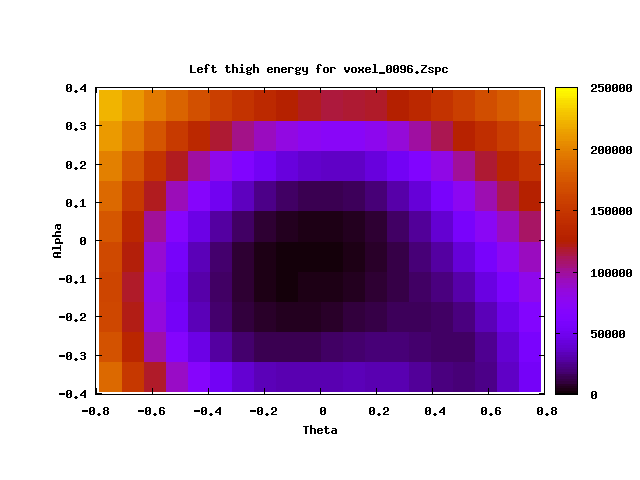
\includegraphics[width=\textwidth]{problems/set81frame96-fixed-leftthigh.png}
	\caption{Energy plot of Frame 96 from Sample 81.
		Darker colours represent lower energies.}
	\label{EnergyPlot}
\end{figure}

We can see from the plot that there is a minimum around the centre - where $(\alpha_1, \theta_1) = (0, 0)$ and the thigh is pointing straight down.

TODO: How do we search for the closest point

